\documentclass[runningheads]{llncs}

\usepackage{iftex}
\ifPDFTeX
  \PackageError{short}{This manuscript must be built with XeLaTeX}{}
\else
  \usepackage{fontspec}
\fi
\usepackage{amsmath,amssymb}
\usepackage{booktabs}
\usepackage{graphicx}
\usepackage{xcolor}
\usepackage{hyperref}
\renewcommand\UrlFont{\color{blue}\rmfamily}
\urlstyle{rm}
\graphicspath{{figures/}}
\emergencystretch=1.5em

\begin{document}

\title{Stress-Testing Product-Gated Clustering and Bounded Priority
Ranking for Flood-Rescue Reports}
\titlerunning{Stress-Testing Flood-Rescue Report Clustering and Ranking}

\author{Anonymous Authors}
\authorrunning{Anonymous Authors}
\institute{Anonymous for review}

\maketitle

\begin{abstract}
Operational flood streams contain duplicate, incomplete, and adversarial
reports, yet clustering and priority scores are often evaluated separately
from scheduling consequences. We study a fail-closed batch pipeline:
receipt-visible reports with location and event time enter a sparse
similarity graph; unresolved reports enter review; deterministic duplicate
families feed a bounded ranking; and evaluator-only truth joins after
predicted-cluster scheduling. The current draft clustering benchmark uses 80
independently seeded synthetic datasets geographically anchored to the
Copernicus EMSR848 activation: 20 development, 20 calibration, and 40 held-out
test runs from one fixed generator regime. Additive Louvain has mean ARI
0.9191, product Leiden 0.9165, and product Louvain 0.9072. The paired
product-minus-additive difference is -0.0118 with bootstrap 95\% CI
[-0.0226,-0.0024], while the Holm-adjusted Wilcoxon result does not establish
a difference ($p=0.1975$). Ranking and scheduling remain part of the proposed
pipeline, but their numerical results are pending dedicated benchmarks.
Neither mathematical boundedness nor this synthetic clustering result implies
policy validity, field benefit, OOD transfer, or misinformation robustness.
\keywords{Flood rescue \and Graph clustering \and Synthetic stress test \and
Priority ranking \and Negative results.}
\end{abstract}

\section{Introduction and Related Work}

Crisis streams mix repeated observations of one event, nearby but distinct
events, missing fields, and nonincident noise. Social-sensor and emergency
message research has long emphasized volume, verification, and event
extraction~\cite{sakaki2010earthquake,atefeh2015survey,imran2015processing}. Multimodal
collections such as CrisisMMD and FloodNet capture important disaster
modalities~\cite{alam2018crisismmd,rahnemoonfar2021floodnet}, but they do not
jointly provide fine-grained physical-incident linkage, rescue priority, and
dispatch outcomes. Consequently, high classification accuracy cannot by
itself establish that a report becomes the right operational destination.

Graph community detection~\cite{blondel2008louvain,traag2019leiden} and
density methods such as DBSCAN, HDBSCAN, and
ST-DBSCAN~\cite{ester1996dbscan,campello2013hdbscan,birant2007stdbscan}
offer plausible consolidation mechanisms. Multiplicative range/domain terms
also occur in bilateral filtering~\cite{tomasi1998bilateral}; we therefore do
not claim a new generic kernel. Spatially constrained clustering and
regionalization encode geography through different objectives
~\cite{chavent2018clustgeo,assuncao2006efficient}. Humanitarian scheduling further exposes
conflicting equity, efficacy, and efficiency objectives
~\cite{gralla2014review,huang2012models,vitoriano2011multicriteria}. A bounded
score is thus a numerical property, not an expert-endorsed rescue policy.

We ask three questions: (RQ1) does independently selected product composition
improve clustering over an additive composition under disclosed search spaces
and one selection rule? (RQ2) does a bounded, duplicate-aware score align with
an independently generated benefit and resist missingness, duplicates,
contradictions, and campaigns? (RQ3) what happens when predicted split, merge,
and noise errors propagate into dispatch rather than being repaired by incident
truth? The present draft populates RQ1 from the available benchmark; RQ2 and
RQ3 remain registered targets pending dedicated experimental outputs.

The contributions are: (i) an observable-only pipeline with explicit review
and evaluator boundaries; (ii) complete product and additive threshold-domain
statements, a component corollary conditional on observed hop diameter, and a
duplicate-aware bounded ranking; and (iii) a development--calibration--held-out
benchmark over 80 synthetic datasets from one fixed generator regime. The main
contribution is diagnostic: mathematical safeguards and held-out synthetic
accuracy must not be converted into deployment claims.

\section{Observable Pipeline and Methods}

Figure~\ref{fig:pipeline} fixes the information boundary. Receipt-visible
fields flow through graph construction, ranking, and a batch scheduler. Missing
location or event time routes a report to review. Incident identity, benefit,
deadline, and harm are stored separately and join only after a schedule exists.

\begin{figure}[t]
\centering
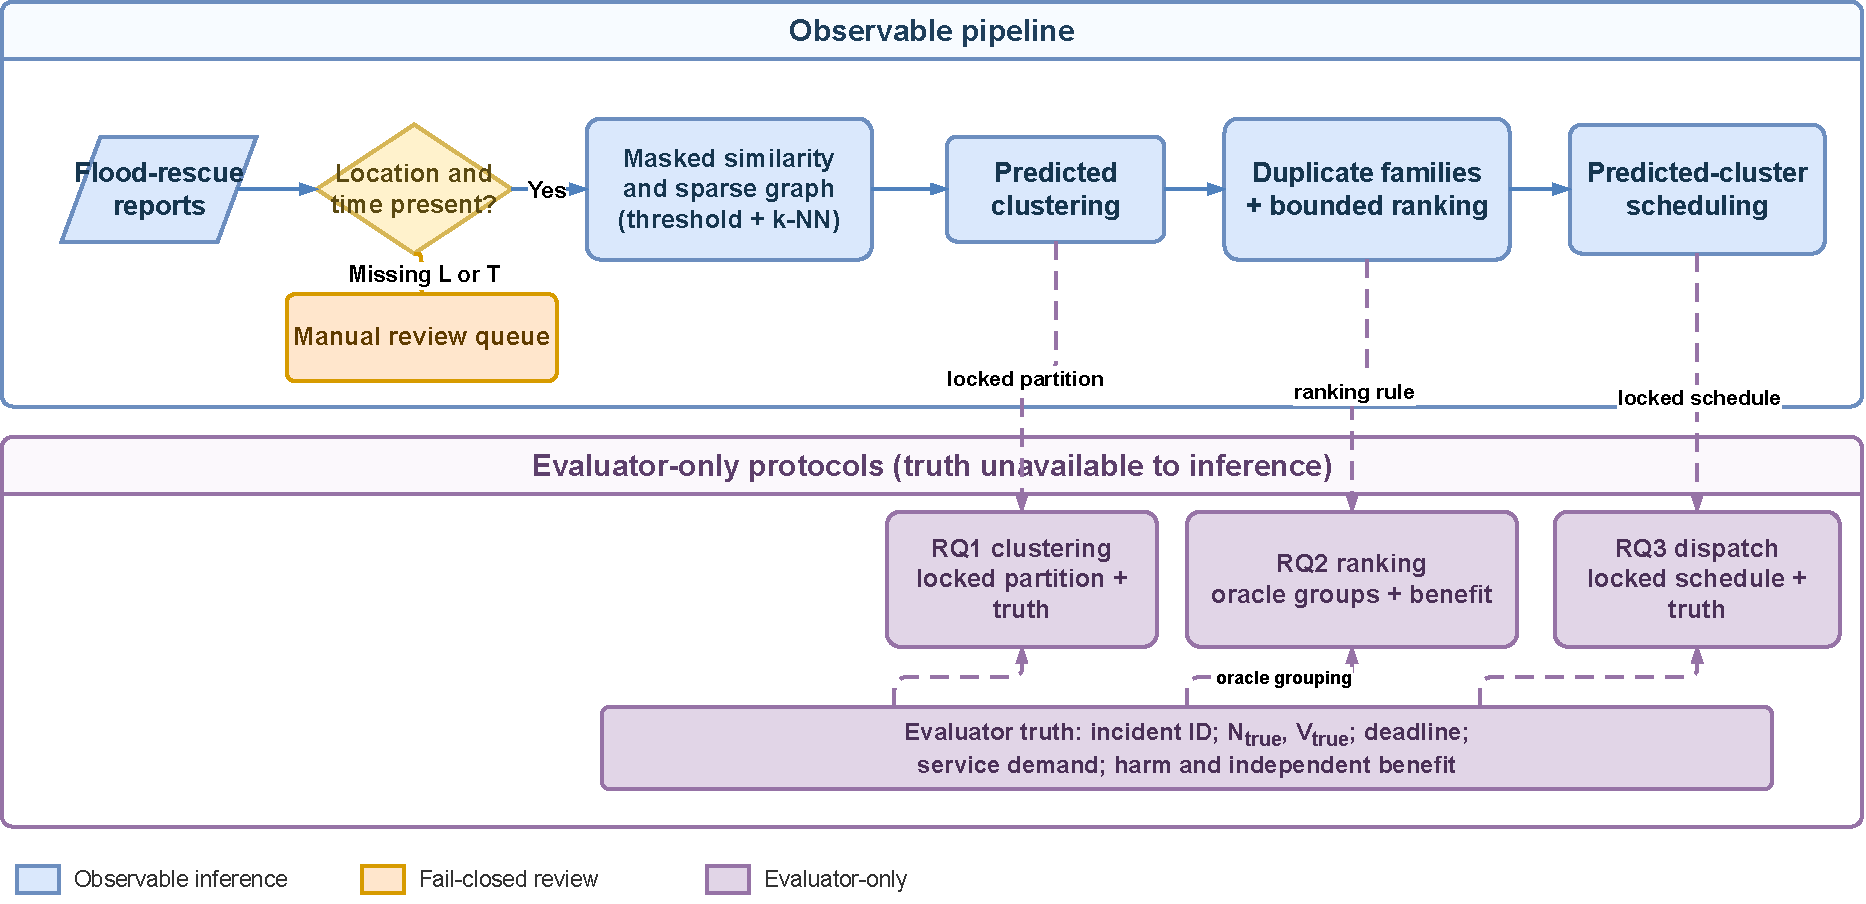
\includegraphics[width=\textwidth]{pipeline_v2.pdf}
\caption{Observable pipeline (solid), manual-review path (orange), and
evaluator-only truth join (dashed). The scheduler receives predicted clusters,
never incident truth.}
\label{fig:pipeline}
\end{figure}

\subsection{Missingness-Aware Similarity and Graph}

A report contains location $L_i$, event time $T_i$, flood evidence $F_i$,
urgency evidence $E_i$, reported demand $N_i$, vulnerability $V_i$, provenance
features, receipt time, and an observation mask. The graph admission indicator
$a_i=\mathbf{1}\{L_i,T_i\text{ are observed}\}$. Thus $a_i a_j=0$ prevents an
edge involving a report whose geographic or temporal separation is undefined;
such a report follows the manual-review path. Missing $F_i$ or $E_i$ is not
zero-imputed: let $I_F(i,j),I_E(i,j)$ indicate that both reports share the
corresponding observation and let $m_{ij}=I_F(i,j)+I_E(i,j)$; then
\[
C_{ij}=\frac{m_{ij}}{2}\exp\!\left[-I_F(i,j)\frac{|F_i-F_j|}{\tau_F}
-I_E(i,j)\frac{|E_i-E_j|}{\tau_E}\right],
\quad C_{ij}=0\ \text{if }m_{ij}=0.
\]
When $m_{ij}=2$, both contextual fields are used; when $m_{ij}=1$, the
maximum contextual similarity is discounted to $1/2$; and when $m_{ij}=0$,
no contextual agreement is inferred. In the current 80-run artifact, every
report has location, event time, flood, and urgency. Hence $a_i=1$ and
$m_{ij}=2$ throughout the evaluated data, reducing the expression to
\[
C_{ij}=\exp\!\left[-\frac{|F_i-F_j|}{\tau_F}
-\frac{|E_i-E_j|}{\tau_E}\right].
\]
The missingness extension is specified and unit-tested, but missingness
robustness is not claimed as an empirical result of this benchmark.
For Haversine distance $d_{ij}$ and time difference $\Delta t_{ij}$, define
\begin{align}
G_{ij}&=\exp[-d_{ij}^{2}/(2\sigma^2)],&
T_{ij}&=\exp[-\Delta t_{ij}/\tau_t],\nonumber\\
w^\times_{ij}&=a_i a_jG_{ij}(\beta T_{ij}+\gamma C_{ij}),&
w^+_{ij}&=a_i a_j(\alpha G_{ij}+\beta T_{ij}+\gamma C_{ij}).
\label{eq:similarities}
\end{align}
All scales $\sigma,\tau_t,\tau_F,\tau_E$ are strictly positive and the
weights are nonnegative. The implementation first forms a common spatial
candidate pool of at most $\max(64,4k)$ neighbours per eligible report,
including all boundary-distance ties before canonical truncation. It computes
an empirical nonzero-weight quantile, retains strict above-threshold edges,
keeps the union of endpoint-wise top-$k$ edges, and applies Louvain. Product
and additive candidates have the same pool and grid, but each family is
selected independently; the estimand is therefore a pipeline comparison, not
an operator-only causal effect.

\begin{theorem}[Product edge localization]
Let $B=\beta+\gamma>0$. If a product edge with threshold $0<\theta<B$ is
retained, then
$d_{ij}<\sigma\sqrt{2\log(B/\theta)}$. For $\theta\ge B$ the strict retained
set is empty; for $\theta\le0$ the threshold alone gives no finite cutoff.
\end{theorem}
\begin{proof}
Since $a_ia_j\le1$ and $T_{ij},C_{ij}\le1$,
$w^\times_{ij}\le B\exp[-d_{ij}^{2}/(2\sigma^2)]$. Combining
$\theta<w^\times_{ij}$ with positivity and taking logarithms gives the bound;
the endpoint cases follow from the same inequality.
\end{proof}
This is an edge statement. A component-diameter claim additionally needs a
bounded observed hop diameter; long transitive chains remain possible.

\begin{corollary}[Conditional component bound]
In the finite product region, a connected component with unweighted observed
hop diameter $h<\infty$ and geographic diameter $D$ satisfies
$D<hr_\theta^\times$, where
$r_\theta^\times=\sigma\sqrt{2\log(B/\theta)}$. A singleton has $h=D=0$.
\end{corollary}
The result follows from the triangle inequality along a path of at most $h$
retained edges. It is a conditional post-hoc component bound, not an ex-ante
compactness guarantee: the pipeline does not control $h$.

For the additive form, assume $\alpha>0$. If
$B<\theta<B+\alpha$, every retained edge satisfies
\[
d_{ij}<r_\theta^+
=\sigma\sqrt{2\log\!\left(\frac{\alpha}{\theta-B}\right)}.
\]
If $\theta\ge B+\alpha$, the strict retained set is empty; if
$\theta\le B$, no non-trivial threshold-induced geographic cutoff exists in
general. Indeed, retention gives
$\theta<\alpha G_{ij}+\beta T_{ij}+\gamma C_{ij}\le\alpha G_{ij}+B$.
Thus product composition has a finite geographic edge bound throughout its
nonempty positive-threshold domain, whereas additive composition has such a
bound only above the maximum non-geographic contribution. Neither statement
alone implies better empirical clustering.

\subsection{Duplicate-Aware Bounded Ranking}

Provenance $Q_i\in[0,1]$ combines a source prior, image presence, and capped
corroboration from distinct source families; proximity alone cannot increase
it. Exact duplicates share a canonical fingerprint. Near duplicates are
merged by deterministic complete linkage, so $A\sim B\sim C$ does not merge
$A$ with $C$ unless every cross-pair passes the envelope.

Let $g$ index the resulting evidence families. Within each family, observed
fields are provenance-gated; across families, demand and vulnerability use
maxima rather than unsupported population sums. In compact form,
\begin{align}
\bar E&=\frac{\sum_g\max_{i\in g}Q_iE_i}
 {\max(1,\sum_g\max_{i\in g}Q_i)},&
\bar F&=\max_{g,i\in g}Q_iF_i,\nonumber\\
\bar N&=\min\!\left(1,\frac{\log(1+\max_{g,i\in g}Q_iN_i)}
 {\log(1+N_{\rm ref})}\right),&
\bar V&=\max_{g,i\in g}Q_iV_i,\nonumber\\
P&=\left[1+(\mu-1)\tanh(\bar V/s)\right]
 (\omega_E\bar E+\omega_F\bar F+\omega_N\bar N).
\label{eq:priority}
\end{align}
Claims are clipped before aggregation. We fix $\omega_E=.40$,
$\omega_F=.35$, $\omega_N=.25$, and $\mu=1.75$; hence
$0\le P\le1.75$. The weights and caps are policy knobs, not learned or
expert-validated parameters. Comparators are a multiplicity-sensitive legacy
score, urgency-only, population-only, a simple linear score, stable random,
and---for dispatch---nearest-first.

\section{Experimental Design}

\paragraph{Data contract and splits.}
The artifact contains 80 independently seeded synthetic datasets
geographically anchored to the Copernicus EMSR848 Central Viet Nam flood
activation. Copernicus EMS, OpenStreetMap, and WorldPop provide geographic or
historical anchors; rescue incidents, reports, duplicates, coordinated
campaigns, vulnerability, and incident labels are synthetic. Every run has 16
latent incidents, 288--370 reports, exact and near duplicates, and three
coordinated nonincident campaigns of 20 reports each. Across all runs are
26,288 reports: 17,901 genuine, 3,587 duplicate, and 4,800 coordinated
nonincident reports. Runs 1--20 are reserved for development, runs 21--40 for
calibration, and runs 41--80 for held-out testing. All runs use one fixed
generator regime, so the experiment measures within-generator variation, not
mechanism-shift OOD transfer. Inference reads only
\texttt{algorithm\_input.json}; ground truth is opened after predictions for a
test run have been produced.

\paragraph{Selection and comparators.}
The current notebook evaluates complete small grids on the 20 calibration
runs and selects mean ARI, breaking ties by standard deviation and canonical
configuration JSON. Product and additive use fixed $\tau_F=.25$,
$\tau_E=.35$, and $\beta=\gamma=.5$. Selected product Louvain uses
$\sigma=700$ m, $\tau_t=60$ min, quantile $.90$, $k=8$, and resolution $1.2$.
Selected additive Louvain uses $\alpha=1$, $\sigma=700$ m, $\tau_t=60$ min,
quantile $.95$, $k=8$, and resolution $1.2$. Because selected quantiles
differ, this is an independently calibrated pipeline comparison, not a
matched-density operator comparison. Comparators are a convex similarity,
product Leiden, geo-time DBSCAN, DBSCAN/HDBSCAN on scaled observable features,
spatially constrained agglomerative clustering, and coordinate K-means. The
implemented geo-time DBSCAN lacks ST-DBSCAN's non-spatial criterion and is
named accordingly.

\paragraph{Endpoints and inference.}
ARI on incident-linked reports~\cite{hubert1985comparing} is the current
primary draft endpoint; NMI, pairwise F1, geographic diameter, and runtime are
descriptive. The existing noise-absorption implementation omits fake-only
clusters from false destinations, so that metric is not reported as evidence.
Before freezing the benchmark, the implementation must add false destinations,
fake absorption, noise rejection, retained-edge fraction, mean degree, and a
matched-density product--additive comparison. Seed-paired ARI differences use
10,000 bootstrap resamples, Wilcoxon signed-rank tests, and Holm correction.
The registered priority stress tests and predicted-cluster dispatch evaluation
remain unchanged in scope, but their numerical results are pending independent
benefit, deadline, service, access-delay, and harm outputs. No clustering
metric is substituted for those outcomes.

\section{Results}

\begin{table}[t]
\centering\small
\caption{Draft held-out clustering snapshot over runs 41--80. ARI uncertainty
is the reported normal-approximation half-width. Lower diameter is descriptive,
not a co-primary endpoint. These values will be replaced after the benchmark
adds matched-density and operational-noise metrics.}
\label{tab:short-clustering-results}
\begin{tabular}{lrrrr}
\toprule
Method & ARI & 95\% half-width & Pair F1 & Mean diam. (km)\\
\midrule
Additive Louvain & \textbf{0.9191} & 0.0197 & \textbf{0.9247} & \textbf{0.3415}\\
Product Leiden & 0.9165 & 0.0190 & 0.9223 & 0.3547\\
Convex Louvain & 0.9135 & 0.0192 & 0.9195 & 0.3547\\
Product Louvain & 0.9072 & 0.0205 & 0.9138 & 0.3585\\
Coordinate K-means & 0.8176 & 0.0203 & 0.8292 & 0.2972\\
Spatial agglomerative & 0.6235 & 0.0269 & 0.6506 & 4.1648\\
HDBSCAN & 0.5205 & 0.0628 & 0.5632 & 1.2527\\
Geo-time DBSCAN & 0.4978 & 0.0390 & 0.5450 & 0.6244\\
DBSCAN, all features & 0.4741 & 0.0471 & 0.5196 & 0.9340\\
\bottomrule
\end{tabular}
\end{table}

Table~\ref{tab:short-clustering-results} gives the current replaceable RQ1
draft. Additive Louvain has the highest mean ARI, followed by product Leiden,
the convex composition, and product Louvain. Product Louvain minus additive
Louvain has mean paired ARI difference $-0.01184$ with bootstrap 95\% CI
$[-0.02257,-0.00240]$: product records 9 wins, 19 ties, and 12 losses. The raw
Wilcoxon $p$ is $0.0987$ and its Holm-adjusted value is $0.1975$. Thus the
registered multiplicity-adjusted test does not establish a product--additive
difference. Product Leiden also does not differ from product Louvain after
Holm adjustment ($p=0.0840$).

The graph compositions have substantially higher held-out ARI than the
current density and agglomerative implementations, but the result is limited
to their disclosed grids and the single authored generator regime. RQ2
priority and RQ3 dispatch tables are intentionally pending. They must not be
filled from the earlier estimated ID/OOD values or inferred from clustering
ARI. The final version will insert results only after dedicated benchmark
artifacts provide independent ranking benefit and scheduling outcomes.

\section{Discussion and Threats to Validity}

The experiment separates mathematical safeguards from empirical benefit.
Product gating localizes retained edges, yet its independently selected
pipeline has a lower mean ARI than additive in the present draft, without a
Holm-significant paired difference. Because product and additive selected
different weight quantiles, their contrast is not an isolated causal effect of
multiplication. A matched-density comparison is required. Likewise, score
boundedness and duplicate-aware aggregation limit numerical influence but do
not by themselves establish source authenticity or priority validity; those
properties still require the registered RQ2 stress tests.

All reports and incident linkage are synthetic. The 40 test runs vary random
seeds inside one generator regime rather than changing mechanisms. The
benchmark therefore provides neither OOD nor field validation. All evaluated
reports contain location, event time, flood, and urgency, so the missingness
extension has not been empirically tested. The current noise metric fails to
count fake-only clusters as false destinations and is omitted until corrected.
No expert panel validated priority weights, caps, or operational utility. No
current result supports ``deployment-ready'', misinformation robustness, or
real-world harm reduction.

\section{Artifact and Conclusion}

The accompanying draft artifact contains the 80-run dataset, benchmark
notebook, calibration grid, selected configurations, per-run test results,
paired comparisons, and editable Figure~\ref{fig:pipeline}. The current table
is a replaceable snapshot. Before submission, every number must be generated
from the accepted CSV and bound to code, data, and configuration hashes.

In conclusion, the complete threshold analysis identifies the finite
geographic domains of product and additive graph weights and makes component
compactness conditional on observed hop diameter. In the current held-out
draft, additive Louvain has the highest mean ARI, but multiplicity-adjusted
paired inference does not establish a difference from product Louvain. The
full observable pipeline, bounded priority ranking, and predicted-cluster
scheduling remain part of the proposed study; their RQ2/RQ3 results await
dedicated benchmark artifacts. The defensible current result is competitive
within-generator clustering plus mathematical audit properties, not policy or
deployment validation.

\bibliographystyle{splncs04}
\bibliography{references}

\end{document}
